\documentclass[class=minimal, border = 0pt, crop]{standalone}
\usepackage{pgf}
\usepackage{tikz}
\usepackage[utf8]{inputenc}
\usetikzlibrary{arrows,automata,shapes,calc, backgrounds}
\usetikzlibrary{positioning}
\pagestyle{empty}
\tikzset{
    state/.style={
           rectangle,
           rounded corners,
           draw=black, very thick,
           minimum height=2em,
           inner sep=5pt,
           text centered,
           },
    pil/.style={
           ->,
           thick,
           shorten <=4pt,
           shorten >=4pt,}
}
\begin{document}
\centering
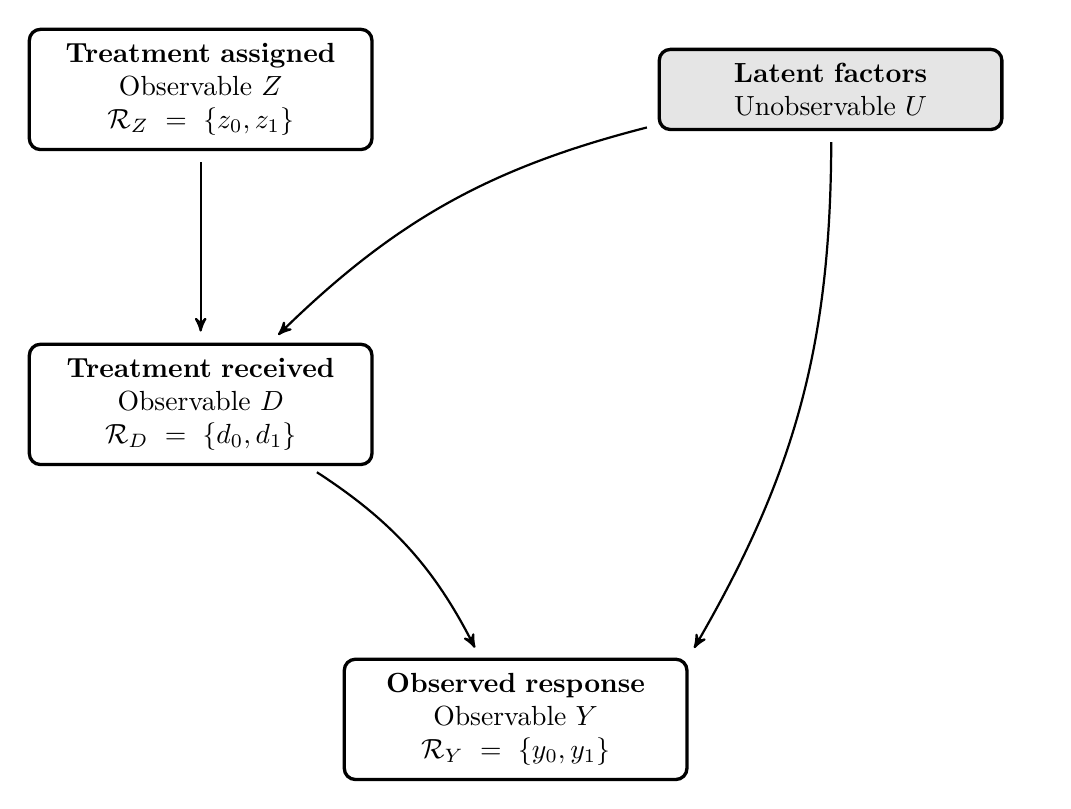
\begin{tikzpicture}[->,>=stealth']
% BASIC MODEL
% Position of Treatment assigned (ASSIGN)
\node[state, text width = 4cm] (ASSIGN)
{
\textbf{Treatment assigned}\\
Observable $Z$\\
$\mathcal{R}_Z=\lbrace z_0,z_1\rbrace$\\
};
% Position of Treatment received (RECEIVE)
\node[state,
text width = 4cm,
below of = ASSIGN,
node distance = 4cm] (RECEIVE)
{\textbf{Treatment received}\\
Observable $D$\\
$\mathcal{R}_D=\lbrace d_0,d_1\rbrace$\\
};
% Position of Observed response (OUTCOME)
\node[state,
text width = 4cm,
below of = RECEIVE,
node distance = 4cm,
xshift = 4cm] (OUTCOME)
{\textbf{Observed response}\\
Observable $Y$\\
$\mathcal{R}_Y=\lbrace y_0,y_1\rbrace$\\
};
% Position of Latent factors (LATENT)
\node[state,
text width = 4cm,
right of = ASSIGN,
node distance = 8cm,
fill = gray!20,
label = right:\phantom{$T$}] (LATENT)
{\textbf{Latent factors}\\
Unobservable $U$\\
};
% Draw lines on graph
\path (LATENT) edge[pil, bend left = 15] (OUTCOME.north east);
\path (LATENT) edge[pil, bend right = 15] (RECEIVE);
\path (ASSIGN) edge[pil] (RECEIVE);
\path (RECEIVE) edge[pil, bend left = 15] (OUTCOME);
%
%
%
%
%
%
%
%
%
%
%
%
%
%
%
%
%
%
%
%
%% Position of Treatment assigned (ASSIGN)
%\node[state, text width = 4cm] (ASSIGN)
%{
%\textbf{Treatment assigned}\\
%Observable $Z$\\
%$\mathcal{R}_Z=\lbrace z_0,z_1\rbrace$\\
%};
%% Position of Treatment received (RECEIVE)
%\node[state,
%text width = 4cm,
%below of = ASSIGN,
%node distance = 4cm] (RECEIVE)
%{\textbf{Treatment received}\\
%Observable $D$\\
%$\mathcal{R}_D=\lbrace d_0,d_1\rbrace$\\
%};
%% Position of Observed response (OUTCOME)
%\node[state,
%text width = 4cm,
%below of = RECEIVE,
%node distance = 4cm,
%xshift = 4cm] (OUTCOME)
%{\textbf{Observed response}\\
%Observable $Y$\\
%$\mathcal{R}_Y=\lbrace y_0,y_1\rbrace$\\
%};
%% Position of Latent factors (LATENT)
%\node[state,
%text width = 4cm,
%right of = ASSIGN,
%node distance = 8cm,
%fill = gray!20,
%label = right:$T$] (LATENT)
%{\textbf{Latent factors}\\
%Unobservable $U$\\
%};
%% Position of Latent factors (LATENT2)
%\node[state,
%text width = 4cm,
%right of = RECEIVE,
%node distance = 8cm,
%fill = gray!20,
%label = right:$R$] (LATENT2)
%{\phantom{\textbf{Latent factors}}\newline
%\phantom{Unobservable $U$}\\
%};
%% Draw lines on graph
%\path (LATENT) edge[pil, bend left = 15] (OUTCOME.north east);
%\path (LATENT) edge[pil, bend right = 15] (RECEIVE);
%\path (ASSIGN) edge[pil] (RECEIVE);
%\path (RECEIVE) edge[pil, bend left = 15] (OUTCOME);
%\node[draw,shape=circle,fill=black,right of = ASSIGN,label=above:$t_1$, node distance = 6.5cm, yshift=-0.15cm] (T1) {};
%\node[draw,shape=circle,fill=black,right of = T1,label=above:$t_2$,node distance = 1cm] (T2) {};
%\node[draw,shape=circle,fill=black,right of = T2,label=above:$t_3$,node distance = 1cm] (T3) {};
%\node[draw,shape=circle,fill=black,right of = T3,label=above:$t_4$,node distance = 1cm] (T4) {};
%\node[draw,shape=circle,fill=black,right of = RECEIVE,label=above:$r_1$, node distance = 6.5cm, yshift=-0.15cm] (R1) {};
%\node[draw,shape=circle,fill=black,right of = R1,label=above:$r_2$,node distance = 1cm] (R2) {};
%\node[draw,shape=circle,fill=black,right of = R2,label=above:$r_3$,node distance = 1cm] (R3) {};
%\node[draw,shape=circle,fill=black,right of = R3,label=above:$r_4$,node distance = 1cm] (R4) {};
\end{tikzpicture}
\end{document}